\documentclass[a4paper,11pt]{ltjsarticle}
\usepackage{amsmath,amssymb}
\usepackage{tikz}
\usetikzlibrary{arrows.meta,angles,quotes}
\usepackage[margin=25mm]{geometry}

\newcommand{\ve}[1]{\boldsymbol{#1}}
\newcommand{\dd}{\mathop{}\!\mathrm{d}}

\title{解析力学（数理）第1回・追加ノート\\極座標の単位ベクトルの時間微分}
\author{}
\date{}

\begin{document}
\maketitle

\noindent\textbf{講義を通して言いたいこと．}
極座標の単位ベクトルは、点の角度 $\theta$ とともに向きを変える。
直交座標の固定基底で表してから微分すると、
$\dot{\ve e}_r=\dot\theta\,\ve e_\theta$ と
$\dot{\ve e}_\theta=-\dot\theta\,\ve e_r$ が得られる。

\medskip
\noindent\small
原典：\texttt{第1回\_追加.pdf}、PDF 1--2ページ。
想定読了時間：約3分（原典の熟読・自力での計算は含まない）。
過去問・演習未確認。詳しさは内容上の必要性で暫定判断した。
\normalsize

\section{極座標の単位ベクトル}

平面上で原点から点への距離を $r$、正の $x$ 軸から測った角度を
$\theta$ とする。固定された直交座標の単位ベクトルを
$\ve e_1,\ve e_2$ と書く。点から外向きに伸びる半径方向の
単位ベクトルを $\ve e_r$、$\theta$ が増える方向を向く接線方向の
単位ベクトルを $\ve e_\theta$ とする。

\begin{center}
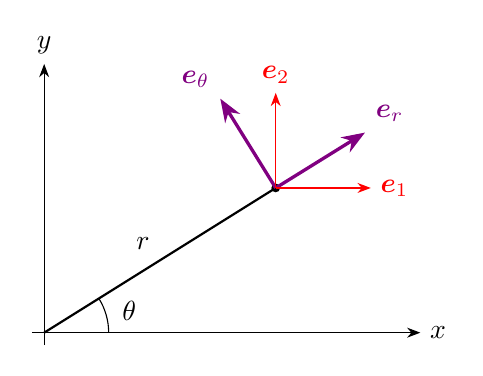
\begin{tikzpicture}[>=Stealth,scale=1.05]
  \coordinate (O) at (0,0);
  \coordinate (P) at (2.8,1.75);
  \draw[->] (-0.15,0) -- (4.55,0) node[right] {$x$};
  \draw[->] (0,-0.15) -- (0,3.25) node[above] {$y$};
  \draw[thick] (O) -- (P) node[midway,above left] {$r$};
  \draw (0.78,0) arc[start angle=0,end angle=32,radius=0.78];
  \node at (1.03,0.26) {$\theta$};
  \fill (P) circle (1.5pt);
  \draw[->,very thick,violet] (P) -- ++(1.08,0.67)
    node[above right] {$\ve e_r$};
  \draw[->,very thick,violet] (P) -- ++(-0.67,1.08)
    node[above left] {$\ve e_\theta$};
  \draw[->,red] (P) -- ++(1.15,0) node[right] {$\ve e_1$};
  \draw[->,red] (P) -- ++(0,1.15) node[above] {$\ve e_2$};
\end{tikzpicture}

\small 図は原典1ページの関係をもとに清書した説明用の図。
\end{center}

\noindent\textbf{方針．}
$\ve e_r,\ve e_\theta$ を時間によらない固定基底
$\ve e_1,\ve e_2$ で表し、その後で時間微分する。
図から各軸への射影を読むと、
\begin{equation}\label{eq:basis}
\boxed{\begin{aligned}
\ve e_r &= \cos\theta\,\ve e_1+\sin\theta\,\ve e_2,\\
\ve e_\theta &= -\sin\theta\,\ve e_1+\cos\theta\,\ve e_2.
\end{aligned}}
\end{equation}
特に $\ve e_\theta$ は $\ve e_r$ を反時計回りに $90^\circ$
回した向きなので、$\ve e_1$ 成分に負号が付く。

\section{時間微分}

角度が時間とともに変化する場合、$\theta=\theta(t)$ と書く。
$\ve e_1,\ve e_2$ は固定基底なので
$\dot{\ve e}_1=\dot{\ve e}_2=\ve 0$ である。
式\eqref{eq:basis}に連鎖律を適用すると、
\begin{align*}
\dot{\ve e}_r
 &= -\sin\theta\,\dot\theta\,\ve e_1
    +\cos\theta\,\dot\theta\,\ve e_2 \\
 &= \dot\theta\bigl(-\sin\theta\,\ve e_1
    +\cos\theta\,\ve e_2\bigr)
  =\boxed{\dot\theta\,\ve e_\theta},\\[4pt]
\dot{\ve e}_\theta
 &= -\cos\theta\,\dot\theta\,\ve e_1
    -\sin\theta\,\dot\theta\,\ve e_2 \\
 &= -\dot\theta\bigl(\cos\theta\,\ve e_1
    +\sin\theta\,\ve e_2\bigr)
  =\boxed{-\dot\theta\,\ve e_r}.
\end{align*}
したがって、求める関係は
\begin{equation}\label{eq:derivative}
\boxed{\dot{\ve e}_r=\dot\theta\,\ve e_\theta,
\qquad
\dot{\ve e}_\theta=-\dot\theta\,\ve e_r.}
\end{equation}

\noindent\textbf{清書時の補足．}
ここでの $\dot\theta=\dd\theta/\dd t$ は角速度である。
$r$ が一定でも $\theta$ が変われば基底は回転するため、
速度や加速度を極座標で求める際には式\eqref{eq:derivative}も微分に含める。

\end{document}
